\section{Описание методов и инструментов для реализации}

\subsection{Система для промышленного интернета вещей}

Как было описано в предыдущим разделе 1,
промышленный анализ данных предоставляет идеи для создания
интеллектуальной системы для автоматизации и повышения
эффективности работы промышленных устройств.
Одной из множества компаний, которая ведет деятельность в данной области,
является компания Omnicube, которая, как уже говорилось,
имеет свою универсальную систему для множества
задач не только промышленного интернета вещей,
но интернета вещей в общем, то есть задачи,
решаемые данной системы, не ограничиваются промышленной отраслью.
Реализация решения для обнаружения и прогнозирования
неисправностей решается в контексте данной системы.
Опишем данную систему.

\begin{figure}[h]
    \center{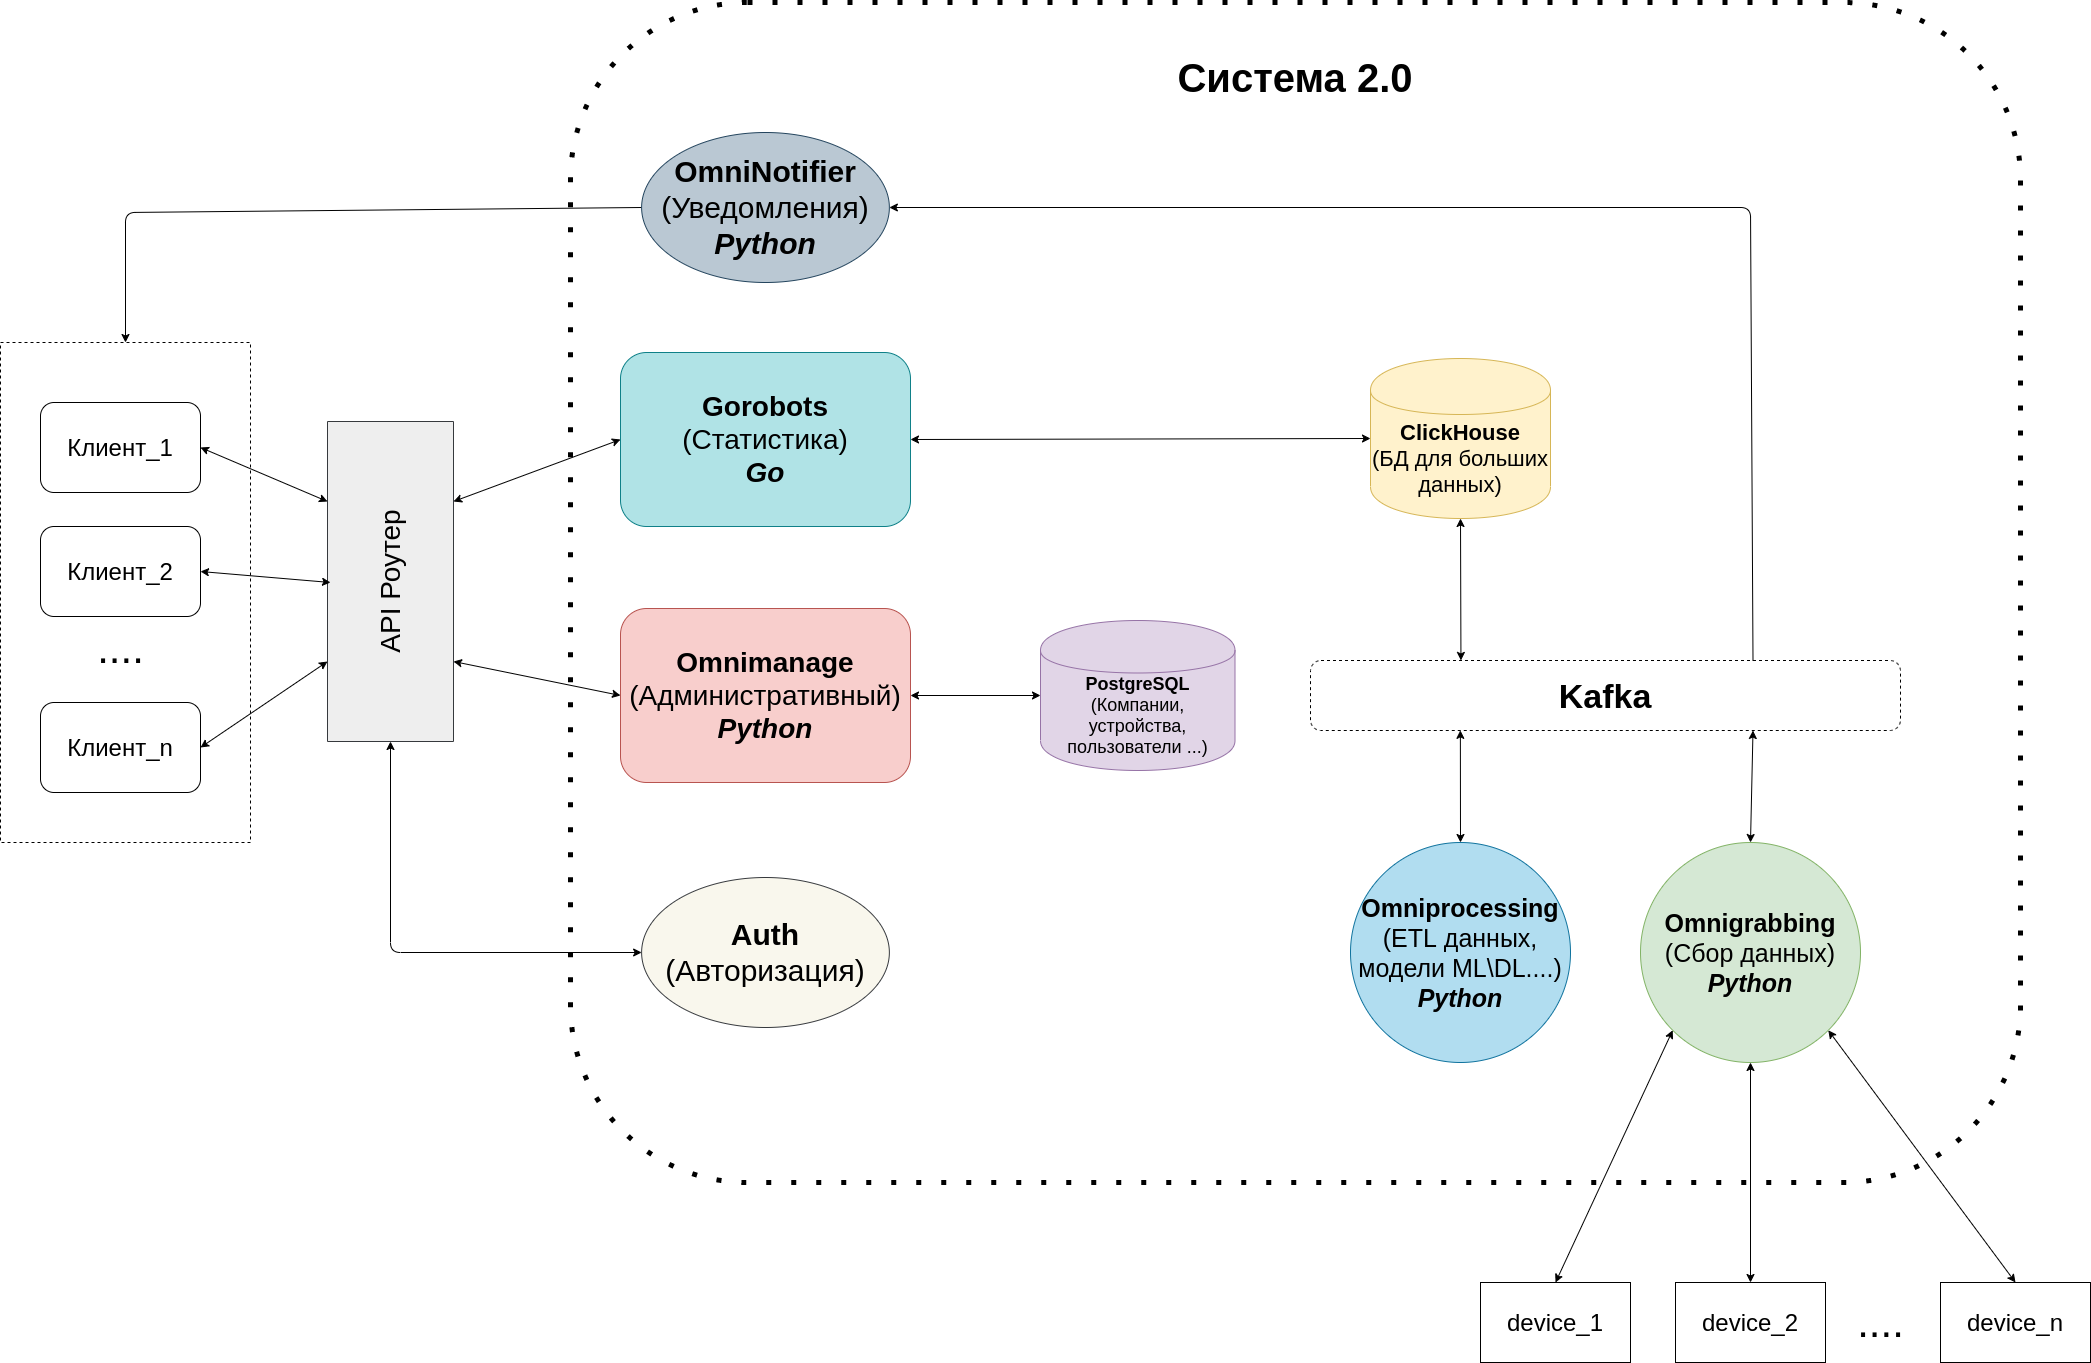
\includegraphics[width=15cm]{img/sys2.png}}
    \caption{Разработанная система для интернета вещей}
\end{figure}

Данная система имеет микросервисную архитектуру.
Микросервисная архитектура представляет собой рассмотрение
разрабатываемого приложения как совокупности связанных сервисов,
каждый их которых отвечает за какую-то часть общей системы,
а также решает свою определенную задачу.
Такой подход имеет свои преимущества и недостатки
Основным преимуществом является модульность,
которая позволяет разрабатывать и поддерживать
компоненты независимо друг от друга.
Недостатками являются:
высокая сложность разработки,
сложный процесс развертывания системы
на собственных кластерах,
и, особенно, на кластерах клиентов.

Основными взаимодействующими с системой структурами являются клиенты и устройства клиентов.
Каждое клиентское устройство соединяется с системой при помощи инженеров компании Omnicube
с учетом специфики самих устройств. Например, для станков лазерной резки Навигатор
использовались датчики, которые устанавливались на критически важные узлы, с которых собиралась необходимая информация.
Помимо этого, сами устройства клиентов иногда предоставляют функционал, который позволяет собирать данные без установки датчиков.
Далее, данные устройств агрегируются и обрабатываются также с учетом специфики устройств.
Обработанные данные выдаются клиентам в виде пользовательского интерфейса, примером которого является
интерфейс для предприятия Сеспель с данными станка лазерной резки Навигатор.

Главными узлами системы являются два микросервиса: omnimanage и gorobots.
Микросервис omnimanage отвечает за обработку первичных данных клиента:
сведения о клиенте, сведения о пользователях компании клиента,
сведения об устройствах клиента (но не сами данные устройств),
сведения о ролях пользователей для авторизации и т.д.
Gorobots отвечает за обработку собранной с устройств
статистики: вычисляет основные статистические показатели (среднее, дисперсию, КПД).
Omnimanage написан на языке Python с использованием базы данных PostgreSQL.
Gorobots написан на языке Go, данные в этом микросервисе берутся из базы данных ClickHouse.

Микросервис omnigrabbing отвечает за сбор и первоначальную обработку данных клиентских устройств.
в данном микросервисе происходит конвертация в необходимых формат для отправления данных в Kafka,
и последующую загрузку в ClickHouse.

Kafka -- платформа для обработки потоковых данных в реальном времени.
Проект направлен на создание унифицированной высокопроизводительной платформы 
с низкой задержкой для обработки потоков данных в реальном времени.
Kafka использует двоичный протокол на основе TCP,
а также системы для обработки асинхронных данных.
Такой брокер был выбран по причине большого количества поступающих данных.
Kafka позволяет гибко решать задачи обработки большого количества асинхронных данных \cite{kafka}.


ClickHouse - это быстрая система управления базами данных OLAP с открытым исходным кодом.
Данная система ориентирована на столбчатую структуру,
а также позволяет генерировать аналитические отчеты с использованием SQL-запросов в режиме реального времени.
База данных была выбрана по причине высокой нагрузки,
заключающейся в необходимости хранить большое количество данных.
Данная СУБД позволяет обрабатывать несколько тысяч запросов в секунду,
что является ключевой особенностью,
которая выделяет данную систему среди других конкурентов \cite{clickhouse}. 

В системе компании Omnicube также присутствуют вспомогательные микросервисы:

\begin{itemize}
    \item API роутер -- система для перенаправления запросов клиентов;
    \item Auth -- сервис для авторизации пользователей;
    \item OmniNotifier -- система для оповещения клиентов.
\end{itemize}

Микросервис omniprocessing является местом, где располагаются различные модели для мониторинга и обработки данных,
например, модели машинного обучения.
Основные цели данного микросервиса -- извлечение, трансформация и загрузка.

В omniprocessing используется Python фреймфорк Faust, который позволяет отправлять
данные в очередь брокеру сообщений Kafka. Из Kafka данные попадают в базу данных ClickHouse.
Благодаря данному фреймворку можно быстро строить и встраивать пайплайны машинного обучения \cite{faust}. 
Разрабатываемое решение для станков Навигатор располагается именно
в микросервисе omniprocessing.

\subsection{Модель выявления признаков}

Основным компонентом системы обнаружения и прогнозирования
неисправностей является модель для кластеризации,
основанная на алгоритме t-Shape.

Среди всех методов, применяемых к данным временных рядов, кластеризация является наиболее широко используемой,
поскольку она не зависит от дорогостоящего человеческого наблюдения или отнимания времени, требующего больших затрат времени. 
С помощью кластеризации возмонжо идентифицировать и обобщить интересные закономерности и корреляции в базовых данных.
В последние несколько десятилетий, кластеризация последовательностей временных рядов получила значительное внимание,
не только как мощный самостоятельный исследовательский метод, но и также как шаг предварительной обработки 
или подпрограмма для других задач. Большинство методов анализа временных рядов, включая кластеризацию, 
критически зависят от выбора меры расстояния. Ключевой вопрос при сравнении двух последовательностей 
временных рядов заключается в том, как обрабатывать различные искажения, 
которые будут обсуждаться, которые характерны для последовательностей.


Из-за этих трудностей и различных потребностей в инвариантности из одной 
области в другую большее внимание уделялось созданию новых мер расстояния, а не созданию новых алгоритмов кластеризации. 
Обычно считается, что выбор меры расстояния более важен, чем сам алгоритм кластеризации. 
Как следствие, кластеризация по временным рядам основывается главным образом на классических методах кластеризации: 
либо путем замены расстояния по умолчанию на более подходящее для временных рядов, 
либо путем преобразования временных рядов в «плоские» данные, чтобы существующие алгоритмы кластеризации 
могут быть использованы непосредственно. Однако выбор метода кластеризации может повлиять: 
на точность, так как каждый метод выражает однородность и разделение кластеров по-разному; и эффективность, 
поскольку вычислительные затраты отличаются от одного метода к другому. Например, спектральная кластеризация 
или некоторые варианты иерархической кластеризации [30] являются более подходящими для идентификации кластеров 
на основе плотности (т. Е. Областей с более высокой плотностью, чем оставшаяся часть данных), 
чем методы разделения, такие как k-средних [30] или к-медоиды [30]. С другой стороны, k-means более эффективен,
чем иерархические, спектральные или k-medoids методы. 

К сожалению, современные подходы к кластеризации на основе форм,
в которых используются методы разбиения с мерами расстояния, не зависящими от масштаба и сдвига, имеют два основных недостатка:
(i) эти подходы не могут масштабироваться до больших объемы данных, поскольку они зависят 
от вычислительно дорогостоящих методов или мер расстояния; 
(ii) эти подходы были разработаны для конкретных доменов или их эффективность была
показана только для ограниченного числа наборов данных. 
Более того, наиболее успешные методы кластеризации на основе форм обрабатывают 
фазовую инвариантность посредством локального нелинейного выравнивания координат 
последовательности, даже если глобальное выравнивание часто является адекватным. 
Например, для набора данных ЭКГ эффективный линейный дрейф может выявить 
основные различия в шаблонах последовательностей двух классов, 
в то время как дорогостоящее нелинейное выравнивание может соответствовать 
каждому соответствующему увеличению или падению каждой последовательности, 
что затрудняет различать два класса. 

Важно отметить, что, насколько известно, эти подходы никогда не подвергались
всесторонней оценке друг против друга, против других методов разделения или против различных подходов, 
таких как иерархические или спектральные методы. 
В статье [31] авторы предложили новый алгоритм k-Shape для кластеризации временных рядов на основе форм, 
который эффективен и не зависит от конкретной системы. k-Shape основан на масштабируемой процедуре итеративного уточнения, 
аналогичной той, которая используется алгоритмом k-средних, но с существенными отличиями. 
В частности, k-Shape использует и другую меру расстояния, и другой метод вычисления центроидов, чем метод k-средних.
Как указывалось выше, k-Shape пытается сохранить формы последовательностей временных рядов при их сравнении. 
Для этого k-Shape требуется мера расстояния, которая инвариантна к масштабированию и сдвигу.
В отличие от других подходов кластеризации,
для k-Shape адаптируется статистическую мера кросс-корреляции

\clearpage

\subsection{Выводы}

В данном разделе был проведен анализ системы компании Omnicube, в которую
будет интегрировано решение для прогнозирования и обнаружения ошибок станков Навигатор.

Кроме этого, был проведен анализ алгоритмов и выбран алгоритм для кластеризации многомерных временных рядов t-Shape.
Именно данный алгоритм поможет качественно определять особенности данных временных рядов станка Навигатор,
и на основе этих особенностей определять обозначенные неисправности.

\clearpage